% Chapter 2

\chapter{Data sources} % Main chapter title

\label{Chapter4} % For referencing the chapter elsewhere, use \ref{Chapter1} 

\lhead{Chapter 4. \emph{Data sources}} % This is for the header on each page - perhaps a shortened title

%----------------------------------------------------------------------------------------
Our application uses two main types of data. \textbf{Static} map data describing the streets and buildings and \textbf{dynamic} data about the different points of interest (POIs). The difference between static and dynamic data lies in the users ability to add and edit POI, while the map information is not meant to be changed by the user.
\par The acquisition of this data was not the essence of the project, so we were allowed to use any data source, with appropriate licence and collaborate with other groups. 

\section{Map data - OpenStreetMap}
Acquisition of map data (roads, road types, buildings etc.) can be extremely time consuming and can easily produce unreliable results. At the same time, there are a lot of different open source data sources available on-line. Together with the other groups we decided to use OpenStreetMap data by the OpenStreetMap Foundation (\cite{osm}).
\par OpenStreetMap is an open source project providing free map data of the world. Data is published under the \textit{Open Database License (ODbL) from Open Data Commons (ODC)}, which enables us to freely produce the works from the database, modify, transform and build upon the database.

\subsection{Data format}
OpenStreetMap data consists of four core elements:
\begin{itemize}
\item \textbf{Nodes} - basic point of location with longitude and latitude information. They can be used to mark a single point (POI) or in a list of nodes (way, relation);
\item \textbf{Ways} - ordered list of nodes, representing a street or an area like a lake, forest etc.;
\item \textbf{Relations} - ordered list of nodes and ways which can be in a relation (many different roads can be part of a long motorway);
\item \textbf{Tags} - key-value pairs which are used to store information about different objects (nodes, ways, relations).
\end{itemize}
Figure \ref{fig:Osm_flow} shows the difference between different core elements
\begin{figure}[h]
\centering
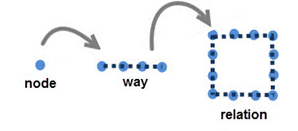
\includegraphics{../pictures/osm_flow.png}
\caption{Representation of basic OSM elements (image taken from \cite{osm_2})}
\label{fig:Osm_flow}
\end{figure}

\section{Points of Interest (POI)}
One of the main requirements for our application is to enable user to search using different points of interest. For acquisition of this points, all of the groups again collaborated, each marking all the points in one part of Le Creusot. For each point we decided to acquire:
\begin{itemize}
\item name;
\item location;
\item address;
\item photo.
\end{itemize}
In the end we also categorized all the points into 26 different categories. 
